\documentclass[10pt]{article}
\usepackage[polish]{babel}
\usepackage[utf8]{inputenc}
\usepackage[T1]{fontenc}
\usepackage{graphicx}
\usepackage[export]{adjustbox}
\graphicspath{ {./images/} }
\usepackage{amsmath}
\usepackage{amsfonts}
\usepackage{amssymb}
\usepackage[version=4]{mhchem}
\usepackage{stmaryrd}

\title{ARKUSZ PRÓBNEJ MATURY Z OPERONEM MATEMATYKA POZIOM ROZSZERZONY }

\author{}
\date{}


\begin{document}
\maketitle
\section*{Czas pracy: 180 minut}
\section*{Instrukcja dla zdającego}
\begin{enumerate}
  \item Sprawdź, czy arkusz egzaminacyjny zawiera 16 stron (zadania 1.-16.). Ewentualny brak zgłoś przewodniczącemu zespołu nadzorującego egzamin.
  \item Rozwiązania zadań i odpowiedzi zapisz w miejscu na to przeznaczonym.
  \item W zadaniach zamkniętych (1,-4.) zaznacz jedną poprawną odpowiedź.
  \item W zadaniu kodowanym (5.) wpisz w tabelę wyniku trzy cyfry wymagane w poleceniu.
  \item W rozwiązaniach zadań otwartych (6.-16.) przedstaw tok rozumowania prowadzący do ostatecznego wyniku.
  \item Pisz czytelnie. Używaj długopisu/pióra tylko z czarnym tuszem/atramentem.
  \item Nie używaj korektora, a błędne zapisy wyraźnie przekreśl.
  \item Zapisy w brudnopisie nie będą oceniane.
  \item Obok numeru każdego zadania podana jest maksymalna liczba punktów możliwych do uzyskania.
  \item Możesz korzystać z zestawu wzorów matematycznych, cyrkla i linijki oraz kalkulatora prostego.\\
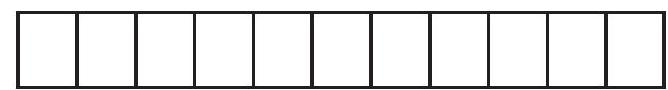
\includegraphics[max width=\textwidth, center]{2024_11_21_e30d1f37bf0e3631c088g-01(1)}
\end{enumerate}

PESEL ZDAJĄCEGO\\
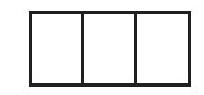
\includegraphics[max width=\textwidth, center]{2024_11_21_e30d1f37bf0e3631c088g-01}

KOD ZDAJĄCEGO

\section*{ZADANIA ZAMKNIĘTE}
W zadaniach od 1. do 4. wybierz poprawną odpowiedź.

\section*{Zadanie 1. (0-1)}
Liczba \(\sqrt{3-2 \sqrt{2}}-\sqrt{9+4 \sqrt{2}}\) jest równa:\\
A. \(-(2-\sqrt{2})\)\\
B. \(-(2+\sqrt{2})\)\\
C. \(-(\sqrt{2}-2)\)\\
D. \(2+\sqrt{2}\)

\section*{Zadanie 2. (0-1)}
Wartość wyrażenia \(\log _{2} 5 \cdot \log _{5} 81 \cdot \log _{9} 216\) wynosi:\\
A. \(6 \log _{2} 6\)\\
B. \(6 \log _{2} 5\)\\
C. \(9 \log _{2} 6\)\\
D. \(6 \log _{2} 9\)

\section*{Zadanie 3. (0-1)}
Równanie \(\left|x^{2}-2 x-8\right|=m+1\) w zależności od parametru \(m\), gdzie \(m \in R\), ma maksymalną liczbę pierwiastków dla:\\
A. \(m \in\langle 0,9)\)\\
B. \(m \in\langle-1,8)\)\\
C. \(m \in(-9,0)\)\\
D. \(m \in(-1,8)\)

\section*{Zadanie 4. (0-1)}
Ciąg \(\left(a_{n}\right)\) jest określony wzorem \(a_{n}=\frac{\left(7 n-n^{2}\right)(3 n+1)}{4 n^{3}+2 n+6}\) dla każdej liczby naturalnej \(n \geq 1\). Granica tego ciągu dla \(n \rightarrow \infty\) jest równa:\\
A. \(\frac{7}{4}\)\\
B. \(-\frac{1}{2}\)\\
C. \(-\frac{3}{4}\)\\
D. \(\frac{1}{2}\)

\section*{BRUDNOPIS (nie podlega ocenie)}
\begin{center}

\includegraphics[max width=\textwidth]{2024_11_21_e30d1f37bf0e3631c088g-03}
\end{center}

\section*{ZADANIA OTWARTE}
\section*{Rozwiązania zadań 5.-16. należy zapisać w wyznaczonych miejscach pod treścią zadania.}
\section*{Zadanie 5. (0-2)}
Rozwiąż nierówność \(\frac{x-6}{36-x^{2}} \geq \frac{3 x}{x^{2}-6 x}\).\\
Wyznacz wszystkie liczby naturalne dodatnie spełniające tę nierówność i oblicz ich iloczyn. W poniższe kratki wpisz kolejno trzy pierwsze cyfry otrzymanego wyniku.\\

\includegraphics[max width=\textwidth, center]{2024_11_21_e30d1f37bf0e3631c088g-04}\\

\includegraphics[max width=\textwidth, center]{2024_11_21_e30d1f37bf0e3631c088g-04(1)}

\section*{Zadanie 6. (0-3)}
Z dwóch podobnych trójkątów prostokątnych o skali podobieństwa 2 zbudowano trapez \(A B C D\). Oblicz miarę kąta ostrego tego trapezu.\\
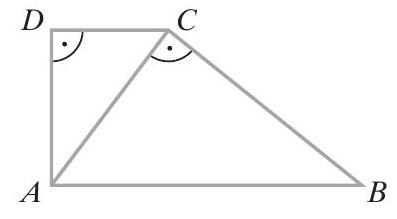
\includegraphics[max width=\textwidth, center]{2024_11_21_e30d1f37bf0e3631c088g-05}\\

\includegraphics[max width=\textwidth, center]{2024_11_21_e30d1f37bf0e3631c088g-05(1)}

Odpowiedź: \(\qquad\)

\section*{Zadanie 7. (0-3)}
Wiesz, że \(a+b+c=0\) i \(a b c=2\). Wykaż, że \(a^{3}+b^{3}+c^{3}=6\).\\

\includegraphics[max width=\textwidth, center]{2024_11_21_e30d1f37bf0e3631c088g-06}

\section*{Zadanie 8. (0-4)}
Reszta z dzielenia wielomianu \(W(x)\) przez dwumian \(x-1\) jest równa 2, a reszta z dzielenia wielomianu \(W(x)\) przez dwumian \(x-2\) jest równa 5 . Wyznacz wielomian \(R(x)\), który jest resztą \(z\) dzielenia wielomianu \(W(x)\) przez \((x-1)(x-2)\).\\

\includegraphics[max width=\textwidth, center]{2024_11_21_e30d1f37bf0e3631c088g-07}

Odpowiedź: \(\qquad\)

\section*{Zadanie 9. (0-4)}
Dany jest czworokąt \(A B C D\), w którym \(|A B|=12,|B C|=6 \sqrt{3},|C D|=3 \sqrt{3},|D A|=3\) i przekątna \(A C\) ma długość 6 . Oblicz długość przekątnej \(B D\) tego czworokąta.

\begin{center}
\begin{tabular}{|c|c|c|c|c|c|c|c|c|c|c|c|c|c|c|c|c|c|c|c|c|}
\hline
 &  &  &  &  &  &  &  &  &  &  &  &  &  &  &  &  &  &  &  &  \\
\hline
 &  &  &  &  &  &  &  &  &  &  &  &  &  &  &  &  &  &  &  &  \\
\hline
 &  &  &  &  &  &  &  &  &  &  &  &  &  &  &  &  &  &  &  &  \\
\hline
 &  &  &  &  &  &  &  &  &  &  &  &  &  &  &  &  &  &  &  &  \\
\hline
 &  &  &  &  &  &  &  &  &  &  &  &  &  &  &  &  &  &  &  &  \\
\hline
 &  &  &  &  &  &  &  &  &  &  &  &  &  &  &  &  &  &  &  &  \\
\hline
 &  &  &  &  &  &  &  &  &  &  &  &  &  &  &  &  &  &  &  &  \\
\hline
 &  &  &  &  &  &  &  &  &  &  &  &  &  &  &  &  &  &  &  &  \\
\hline
 &  &  &  &  &  &  &  &  &  &  &  &  &  &  &  &  &  &  &  &  \\
\hline
 &  &  &  &  &  &  &  &  &  &  &  &  &  &  &  &  &  &  &  &  \\
\hline
 &  &  &  &  &  &  &  &  &  &  &  &  &  &  &  &  &  &  &  &  \\
\hline
 &  &  &  &  &  &  &  &  &  &  &  &  &  &  &  &  &  &  &  &  \\
\hline
 &  &  &  &  &  &  &  &  &  &  &  &  &  &  &  &  &  &  &  &  \\
\hline
 &  &  &  &  &  &  &  &  &  &  &  &  &  &  &  &  &  &  &  &  \\
\hline
 &  &  &  &  &  &  &  &  &  &  &  &  &  &  &  &  &  &  &  &  \\
\hline
 &  &  &  &  &  &  &  &  &  &  &  &  &  &  &  &  &  &  &  &  \\
\hline
 &  &  &  &  &  &  &  &  &  &  &  &  &  &  &  &  &  &  &  &  \\
\hline
 &  &  &  &  &  &  &  &  &  &  &  &  &  &  &  &  &  &  &  &  \\
\hline
 &  &  &  &  &  &  &  &  &  &  &  &  &  &  &  &  &  &  &  &  \\
\hline
 &  &  &  &  &  &  &  &  &  &  &  &  &  &  &  &  &  &  &  &  \\
\hline
 &  &  &  &  &  &  &  &  &  &  &  &  &  &  &  &  &  &  &  &  \\
\hline
 &  &  &  &  &  &  &  &  &  &  &  &  &  &  &  &  &  &  &  &  \\
\hline
 &  &  &  &  &  &  &  &  &  &  &  &  &  &  &  &  &  &  &  &  \\
\hline
 &  &  &  &  &  &  &  &  &  &  &  &  &  &  &  &  &  &  &  &  \\
\hline
 &  &  &  &  &  &  &  &  &  &  &  &  &  &  &  &  &  &  &  &  \\
\hline
 &  &  &  &  &  &  &  &  &  &  &  &  &  &  &  &  &  &  &  &  \\
\hline
 &  &  &  &  &  &  &  &  &  &  &  &  &  &  &  &  &  &  &  &  \\
\hline
 &  &  &  &  &  &  &  &  &  &  &  &  &  &  &  &  &  &  &  &  \\
\hline
 &  &  &  &  &  &  &  &  &  &  &  &  &  &  &  &  &  &  &  &  \\
\hline
 &  &  &  &  &  &  &  &  &  &  &  &  &  &  &  &  &  &  &  &  \\
\hline
 &  &  &  &  &  &  &  &  &  &  &  &  &  &  &  &  &  &  &  &  \\
\hline
 &  &  &  &  &  &  &  &  &  &  &  &  &  &  &  &  &  &  &  &  \\
\hline
 &  &  &  &  &  &  &  &  &  &  &  &  &  &  &  &  &  &  &  &  \\
\hline
 &  &  &  &  &  &  &  &  &  &  &  &  &  &  &  &  &  &  &  &  \\
\hline
 &  &  &  &  &  &  &  &  &  &  &  &  &  &  &  &  &  &  &  &  \\
\hline
 &  &  &  &  &  &  &  &  &  &  &  &  &  &  &  &  &  &  &  &  \\
\hline
 &  &  &  &  &  &  &  &  &  &  &  &  &  &  &  &  &  &  &  &  \\
\hline
 &  &  &  &  &  &  &  &  &  &  &  &  &  &  &  &  &  &  &  &  \\
\hline
 &  &  &  &  &  &  &  &  &  &  &  &  &  &  &  &  &  &  &  &  \\
\hline
 &  &  &  &  &  &  &  &  &  &  &  &  &  &  &  &  &  &  &  &  \\
\hline
\end{tabular}
\end{center}

Odpowiedź: \(\qquad\)\\
8

\section*{Zadanie 10. (0-2)}
Dana jest funkcja \(f\) określona wzorem \(f(x)=\frac{9-4 x^{2}}{x^{2}+1}\). Oblicz wartość pochodnej tej funkcji dla\\
argumentu -3 .\\

\includegraphics[max width=\textwidth, center]{2024_11_21_e30d1f37bf0e3631c088g-09}

Odpowiedź:

\section*{Zadanie 11. (0-3)}
Wyznaczrównania stycznych do okręgu \(x^{2}+y^{2}-2 x-8=0\) równoległych do prostej \(y=2 x+5\).\\

\includegraphics[max width=\textwidth, center]{2024_11_21_e30d1f37bf0e3631c088g-10}

Odpowiedź:

10

\section*{Zadanie 12. (0-5)}
Rozwiąż równanie \(2 \sin ^{3} x-\sin x \cos x-\sin x=0 \mathrm{w}\) przedziale \(\langle 0,2 \pi\rangle\).\\

\includegraphics[max width=\textwidth, center]{2024_11_21_e30d1f37bf0e3631c088g-11}

Odpowiedź: \(\qquad\)

\section*{Zadanie 13. (0-4)}
Wyznacz wszystkie wartości parametru \(m\), dla których trójmian kwadratowy\\
\(f(x)=-x^{2}+m x-m\) ma dwa różne pierwiastki rzeczywiste \(x_{1}\) i \(x_{2}\), spełniające warunek \(\left(x_{1}+3 x_{2}\right)\left(x_{2}+3 x_{1}\right)=-1\).\\

\includegraphics[max width=\textwidth, center]{2024_11_21_e30d1f37bf0e3631c088g-12}

Odpowiedź:\\
12

\section*{Zadanie 14. (0-5)}
Z urny zawierającej 6 kul białych i 4 kule czarne losujemy 2 kule i wkładamy je do drugiej, pustej urny. Następnie z obu urn losujemy po jednej kuli. Oblicz prawdopodobieństwo, że będą to dwie kule czarne.\\

\includegraphics[max width=\textwidth, center]{2024_11_21_e30d1f37bf0e3631c088g-13}

Odpowiedź: \(\qquad\)

\section*{Zadanie 15. (0-4)}
Między liczby 4 i 36 wstawiono trzy liczby tak, aby w utworzonym w ten sposób ciągu trzy pierwsze liczby tworzyły ciąg arytmetyczny, a trzy ostatnie - ciąg geometryczny i aby suma wszystkich pięciu liczb wynosiła 90 . Wyznacz te liczby.\\

\includegraphics[max width=\textwidth, center]{2024_11_21_e30d1f37bf0e3631c088g-14}

Odpowiedź: \(\qquad\)

\section*{Zadanie 16. (0-7)}
Suma długości krawędzi graniastosłupa prawidłowego czworokątnego wynosi \(12 \sqrt{3}\). Wyznacz największą z możliwych objętość tego graniastosłupa. Wynik zapisz w najprostszej postaci.\\

\includegraphics[max width=\textwidth, center]{2024_11_21_e30d1f37bf0e3631c088g-15}

Odpowiedź:

\section*{BRUDNOPIS (nie podlega ocenie)}

\includegraphics[max width=\textwidth, center]{2024_11_21_e30d1f37bf0e3631c088g-16(1)}\\
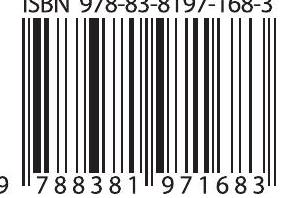
\includegraphics[max width=\textwidth, center]{2024_11_21_e30d1f37bf0e3631c088g-16}

16


\end{document}